\documentclass[12pt]{article}
\usepackage[brazil]{babel}
\usepackage[a4paper, total={6.5in, 9.5in}]{geometry}
\usepackage[utf8]{inputenc}
\usepackage[T1]{fontenc}
\usepackage{listings}
\usepackage{xcolor}
\usepackage{float}
\usepackage{graphicx}
\usepackage{hyperref}
\usepackage{lipsum}
\usepackage{amsmath}
\usepackage[normalem]{ulem}

\definecolor{codegreen}{rgb}{0,0.6,0}
\definecolor{codegray}{rgb}{0.5,0.5,0.5}
\definecolor{codered}{rgb}{0.8,0,0}
\definecolor{backcolour}{rgb}{0.95,0.95,0.92}

\usepackage{inconsolata}
\lstset{
    language=php,
    backgroundcolor=\color{backcolour},   
    commentstyle=\color{codegreen},
    keywordstyle=\color{blue},
    numberstyle=\tiny\color{codegray},
    stringstyle=\color{codered},
    basicstyle=\ttfamily\small,
    numberstyle=\footnotesize,
    numbers=left,
    backgroundcolor=\color{gray!10},
    frame=single,
    tabsize=2,
    rulecolor=\color{black!30},
    title=\lstname,
    escapeinside={\%*}{*)},
    breaklines=true,
    breakatwhitespace=true,
    framextopmargin=2pt,
    framexbottommargin=2pt,
    inputencoding=utf8,
    extendedchars=true,
    showstringspaces=false,
    literate={á}{{\'a}}1 {ã}{{\~a}}1 {é}{{\'e}}1 {Ó}{{\'O}}1 {Ã}{{\~A}}1 {í}{{\'i}}1 {ó}{{\'o}}1,
}

\title{Projeto Final}
\author{Pedro Henrique de Brito Agnes, 18/0026305 \\
Pedro Pessoa Ramos, 18/0026488}
\date{}

\begin{document} 
\maketitle

\section*{Introdução}
Para o projeto final da disciplina de Banco de Dados, foi desenvolvido um \textit{software} com o objetivo de auxiliar o professor no modelo de aulas remotas. Neste sistema, o professor seria capaz de consultar a acessibilidade dos alunos a recursos como internet, computador, dispositivos móveis, o que permite avaliar a situação de seus alunos para encontrar um formato de aula que não os prejudique. Também, entre diversas outras possibilidades, é possível manter registros da participação dos alunos em cada aula, seja síncrona ou assíncrona, já que pode cadastrar os tipos de participação como fazer exercícios e assistir a aula.

\section*{Detalhes Técnicos}
Foram usadas a linguagem de programação PHP e um banco de dados com o SGBD MySQL para o desenvolvimento do sistema. Para a implementação da interface de usuário, foi desenvolvida uma API que serve como o CRUD do projeto, responsável por acessar cada tabela do banco para as operações de inserção, atualização, remoção e consulta. Já no banco, foram criadas 10 entidades, que totalizaram 13 tabelas seguindo o modelo proposto para aulas remotas, como informações do aluno, professor, participação das aulas, plataformas em que as aulas são dadas, entre outros.

O CRUD do projeto está funcionando em um servidor web e pode ser acessado pelo link \url{https://api2.opessoa.com.br/ProjetoBD}, assim como o banco também está no mesmo domínio. Após acessar o link, uma resposta no formato JSON deve ser recebida informando um erro, pois não foi informada uma classe. Existe uma classe para cada tabela, chamadas de \textit{controllers}, que efetuam as operações de manipulação e consulta dos dados da tabela conforme solicitado pelo usuário. Como exemplo, se quisermos acessar o \textit{controller} dos alunos, podemos chamar o \texttt{AlunosController} e, em seguida, a função que queremos utilizar dele, que são as mesmas para cada um: \texttt{get}, \texttt{insert}, \texttt{delete} e \texttt{update} (\pageref{operacoes}).

O padrão de nomenclatura dos \textit{controllers} é o nome da tabela em plural seguido por "\textit{Controller}" e usando \textit{camel case} para tabelas de nome composto como as de relacionamento. Acima foi mostrado como utilizar o comando \texttt{SELECT}, porém os comandos \texttt{INSERT}, \texttt{DELETE} e \texttt{UPDATE} precisam de parâmetros adicionais, que são os valores de cada coluna a inserir e no caso de excluir, devem ser passadas todas as chaves primárias, tudo separado por \texttt{/} e na ordem vista durante o \texttt{SELECT}. Já no update, são passadas todas as chaves assim como na remoção e, em seguida os parâmetros a serem alterados na ordem, assim como na inserção. Posteriormente serão mostrados exemplos de como efetuar cada operação (\pageref{operacoes}).

\subsection*{Modelo Entidade Relacionamento}
A seguir, podemos ver o MER do projeto, que retrata a ideia inicial do projeto, onde foram pensados e diagramados os relacionamentos, as entidades e os atributos e chaves primárias de cada. Aqui foi onde começou a estrutura do banco de dados desenvolvido.

\begin{figure}[H]
	\centering
    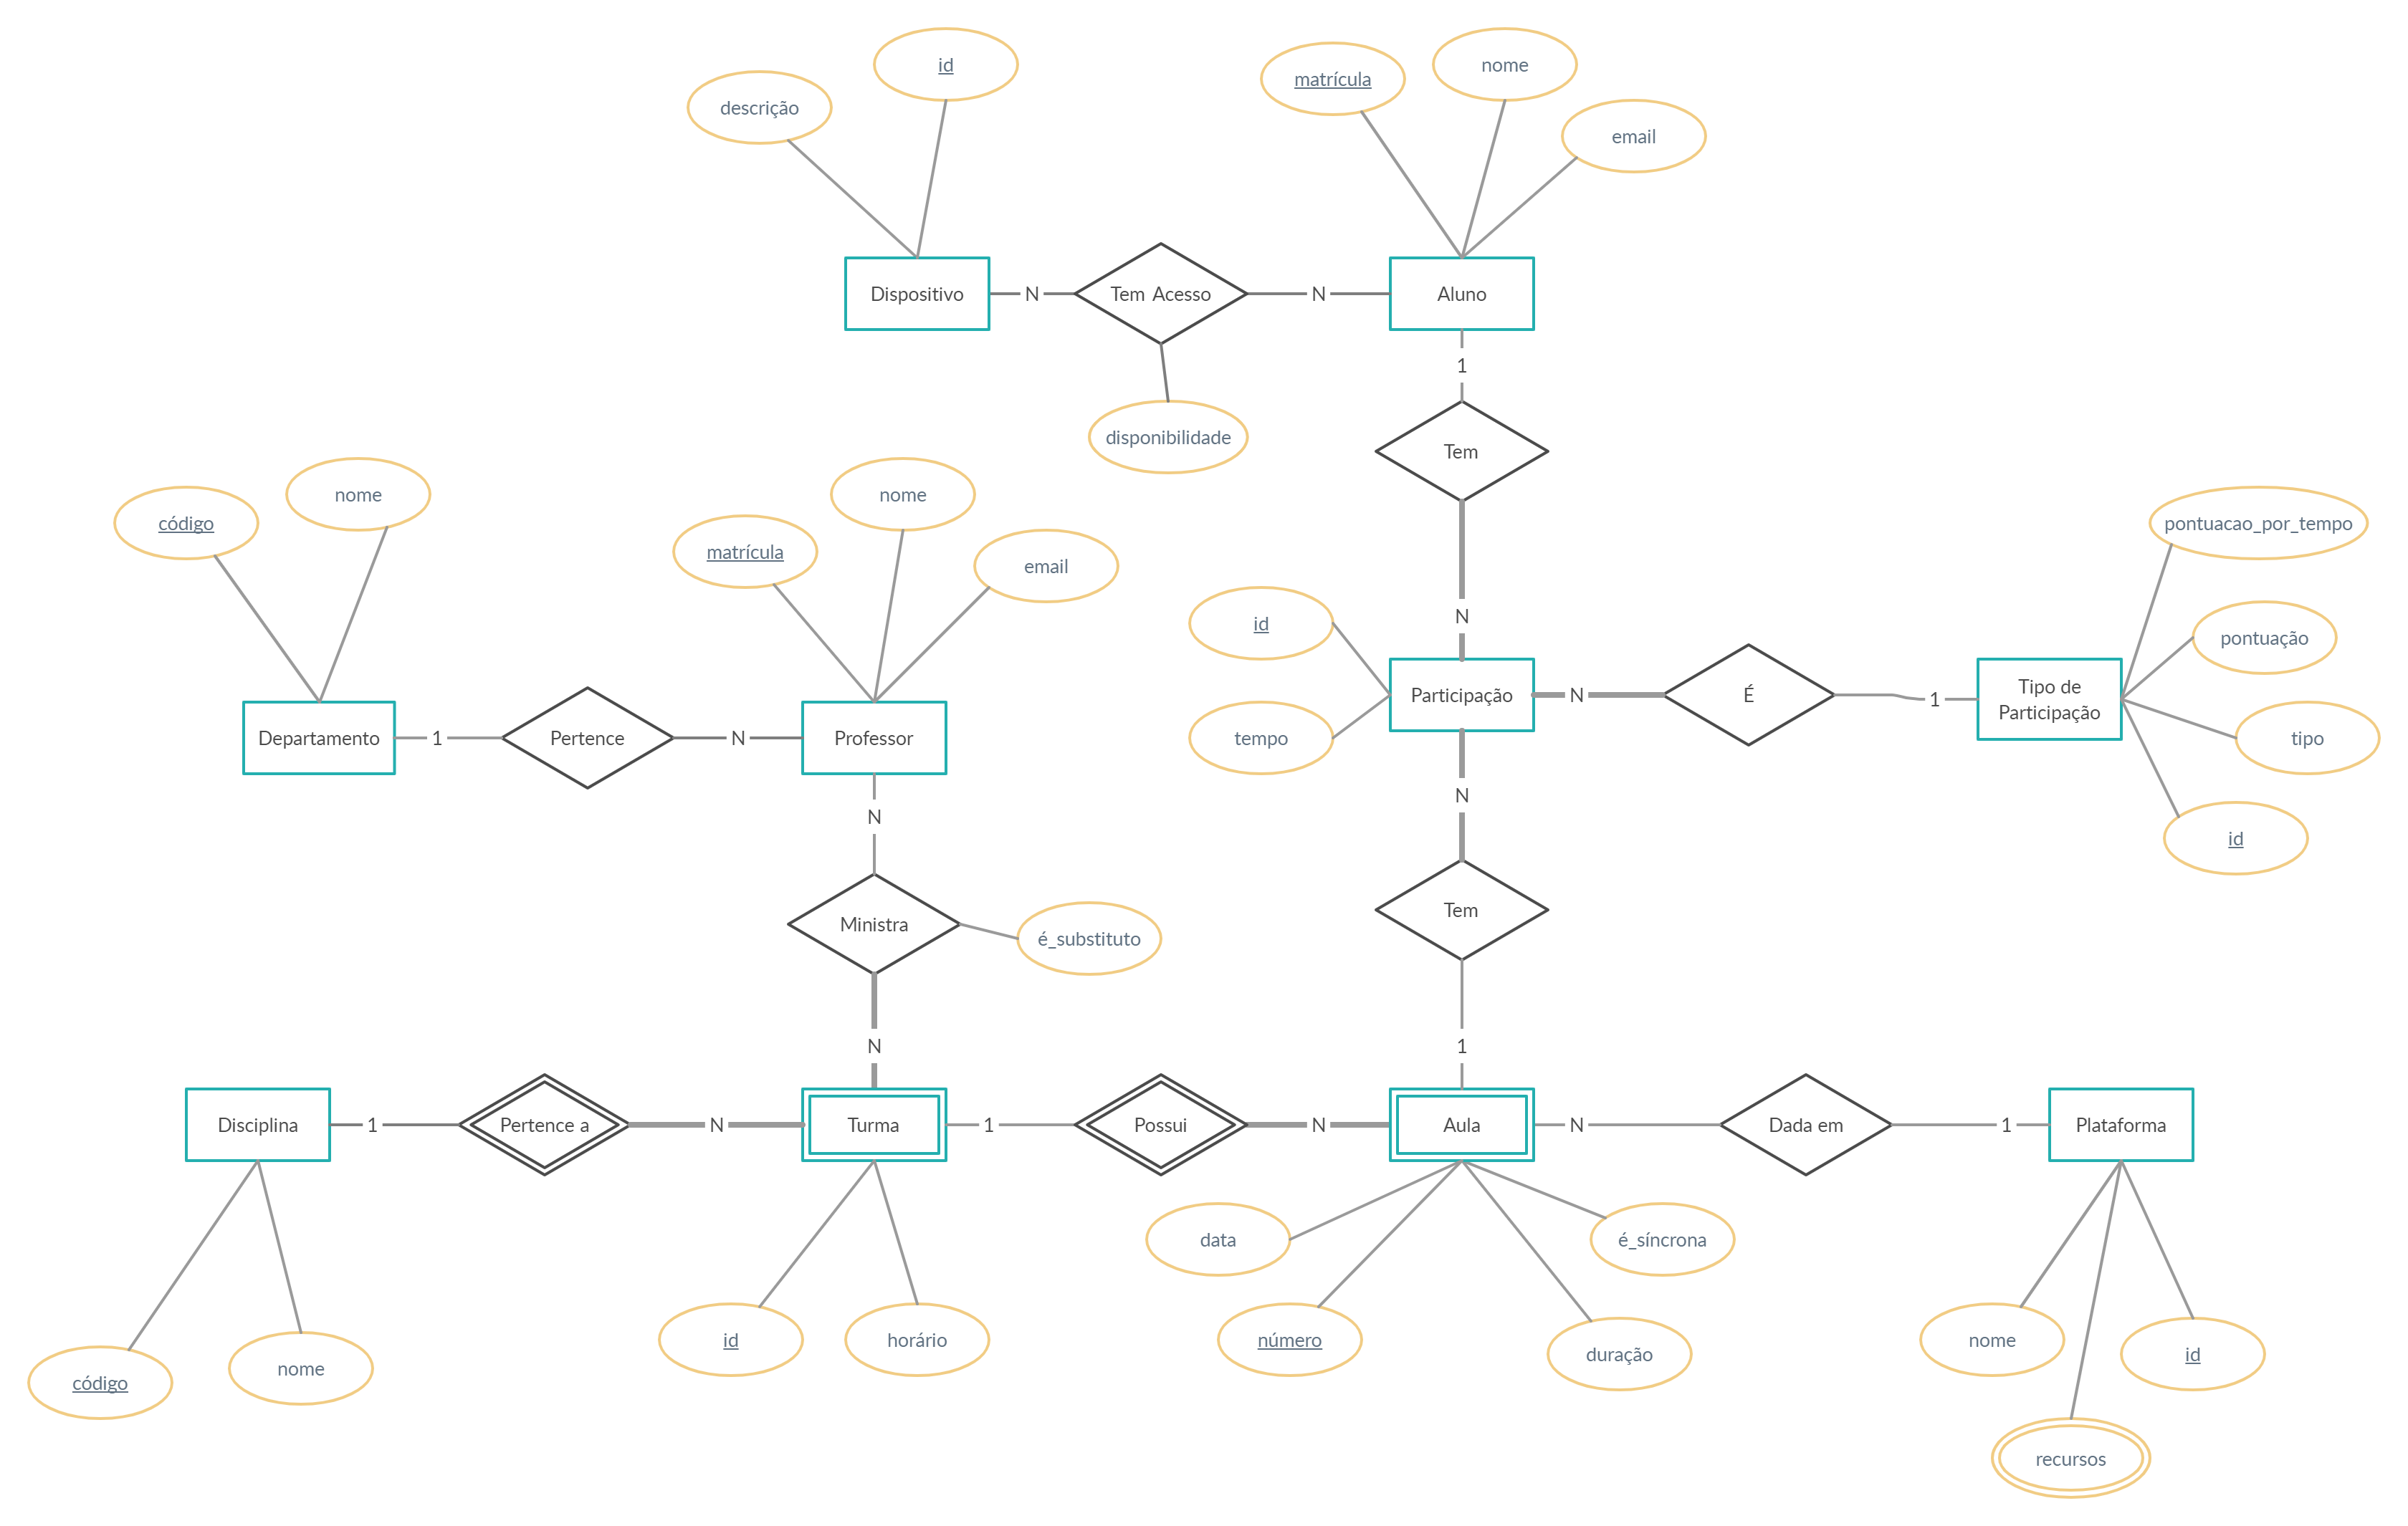
\includegraphics[width=1\textwidth]{MER.png}
    \caption{Modelo Entidade Relacionamento}
\end{figure}

\textbf{Lista de entidades:}
\begin{itemize}
    \setlength\itemsep{0.1em}
    \item Aluno
    \item Aula
    \item Departamento
    \item Disciplina
    \item Dispositivo
    \item Participação
    \item Plataforma
    \item Professor
    \item Tipo de Participação
    \item Turma
\end{itemize}

\newpage

\subsection*{Modelo Relacional}
Abaixo podemos ver o MR do projeto, onde foram especificados detalhes mais internos ao banco como os tipos de cada atributo e a organização das chaves estrangeiras e tabelas de relacionamento, assim como as tabelas para atributos multivalorados. Aqui foi onde começou a implementação do banco de dados desenvolvido. Na página \pageref{mapeamento-controller}, pode ser encontrada a lista completa das tabelas do banco, assim como o mapeamento de cada uma para a respectiva classe controladora.

\begin{figure}[H]
	\centering
    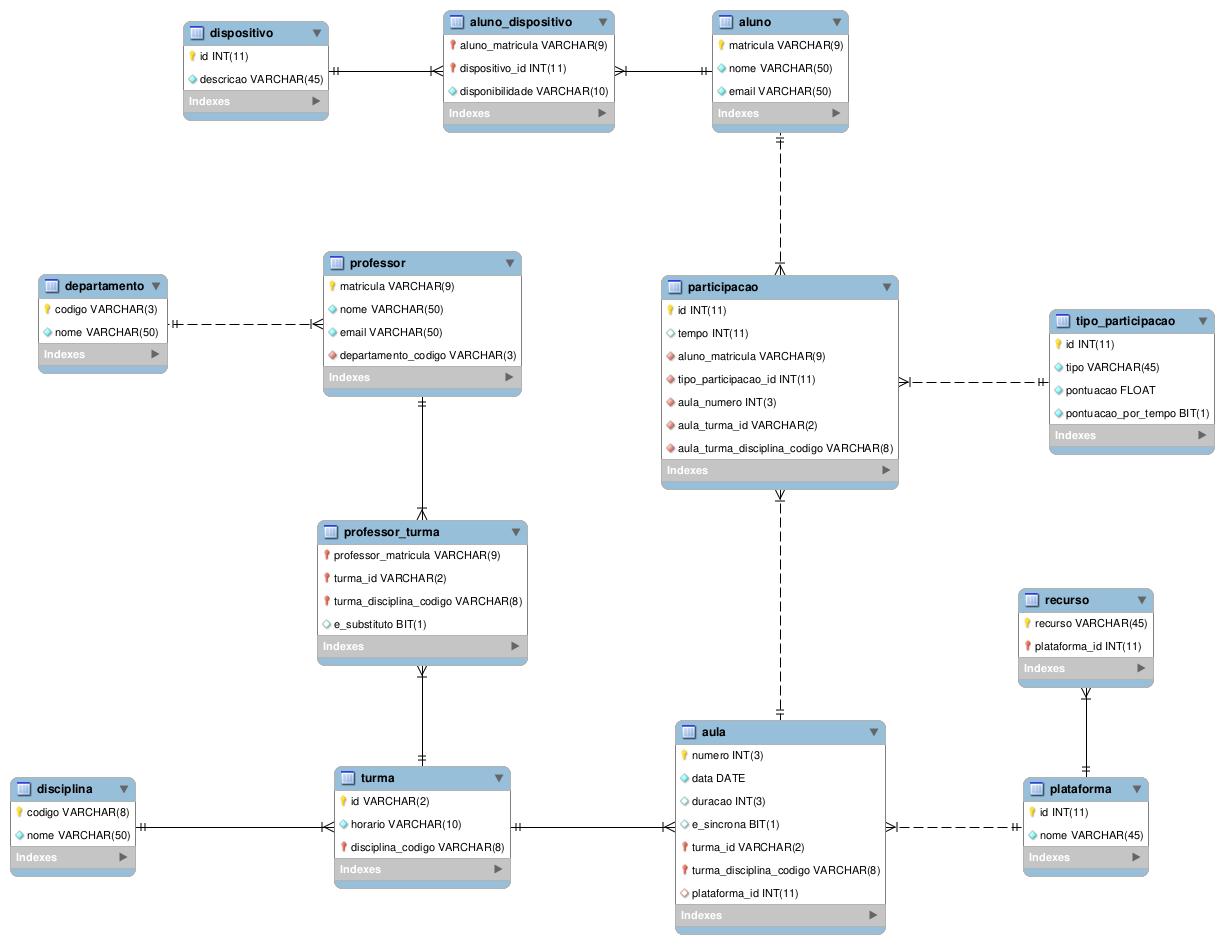
\includegraphics[width=1\textwidth]{MR.png}
    \caption{Modelo Relacional}
\end{figure}

\section*{Álgebra Relacional}
\textbf{Todas as combinações possíveis de alunos, dispositivos, e participação.}

\begin{equation}
    dispositivo \times aluno \times tipo\_participacao
\end{equation}

\noindent \textbf{Todas as pessoas cadastradas (alunos e professores) mais o departamento do professor e dispositivo do aluno.}

\begin{equation}
\begin{split}
    \sigma_{aluno.matricula = aluno\_dispositivo.aluno\_matricula\ AND\ dispositivo.id = aluno\_dispositivo.dispositivo\_id} \\
    (aluno \times aluno\_dispositivo \times dispositivo) \cup (professor \bowtie departamento)
\end{split}
\end{equation}

\noindent \textbf{Relação de professor com turma.}

\begin{equation}
    professor \bowtie professor\_turma \bowtie turma
\end{equation}

\noindent \textbf{Todas as possíveis formas de passar aulas.}

\begin{equation}
    tipo\_participacao \times plataforma \times recurso
\end{equation}

\noindent \textbf{Disciplinas que não tiveram aulas.}

\begin{equation}
    \sigma_{disciplina.codigo\ not\ in\ aula.turma\_disciplina\_codigo}(disciplina \bowtie aula)
\end{equation}

\section*{Forma Normal}
Avaliação das formas normais em cinco tabelas (\textbf{PEDRO PESSOA}).

\newpage

\section*{Camada de Persistência}
Abaixo temos um diagrama mostrando como a interface da API por meio da classe \texttt{mysqli} do php extendida por \texttt{Conn} no projeto acessa o banco de dados para realizar as operações do CRUD. Logo abaixo, temos uma tabela de mapeamento de cada tabela do banco para a respectiva classe controladora.

\begin{figure}[H]
    \centering
    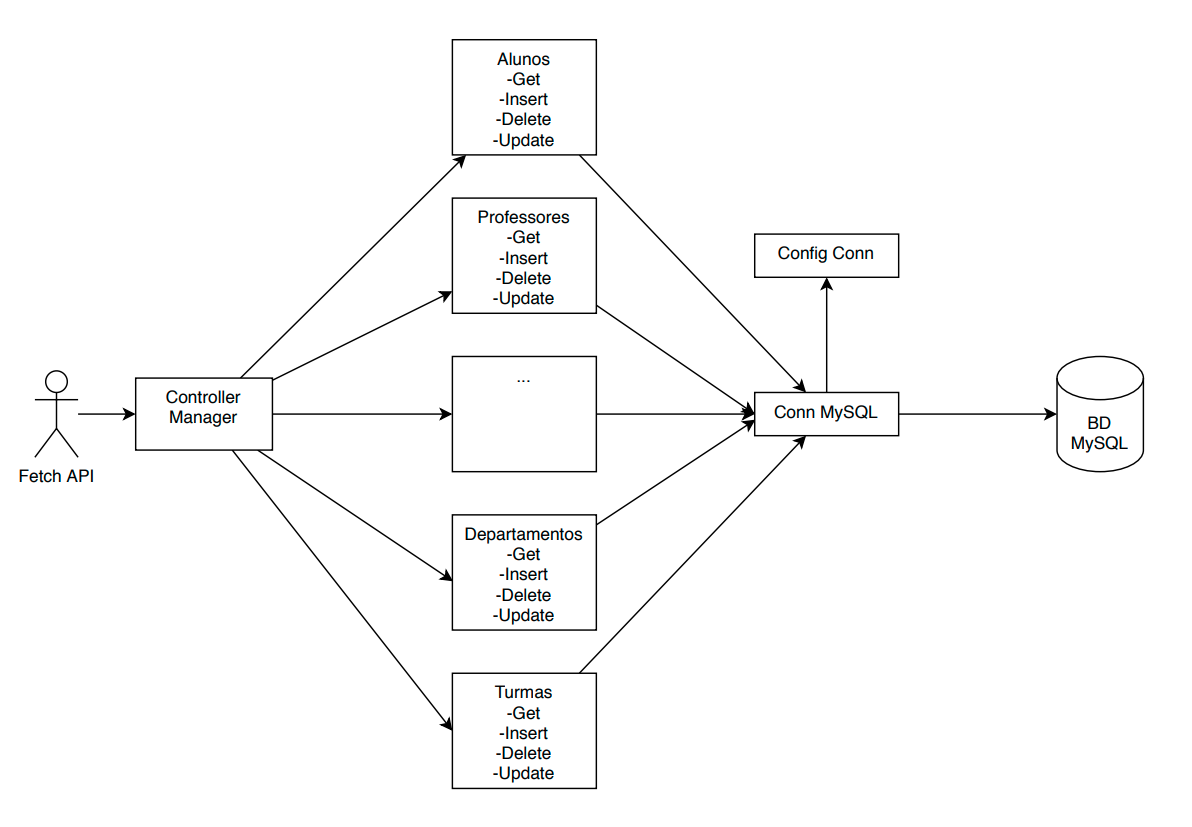
\includegraphics[width=1\textwidth]{diagrama_persistencia.png}
    \caption{Diagrama de acesso a camada de persistência}
\end{figure}

\begin{center}
    \begin{tabular}{|p{.45\textwidth}|p{.45\textwidth}|}
        \hline
        \textbf{Tabela} & \textbf{\textit{Controller}} \\
        \hline
        aluno & AlunosController \\
        \hline 
        aluno\_dispositivo & AlunosDispositivosController \\
        \hline  
        aula & AulasController \\
        \hline 
        departamento & DepartamentoController \\
        \hline
        disciplina & DisciplinasController \\
        \hline
        dispositivo & DispositivosController \\
        \hline
        participacao & ParticipacoesController \\
        \hline
        plataforma & PlataformasController \\
        \hline
        professor & ProfessoresController \\
        \hline
        professor\_turma & ProfessoresTurmasController \\
        \hline
        recurso & RecursosController \\
        \hline
        tipo\_participacao & TiposParticipacaoController \\
        \hline
        turma & TurmasController \\
        \hline
    \end{tabular}\label{mapeamento-controller}
\end{center}

\subsection*{Exemplos das Operações na tabela de Alunos}
É importante mencionar que nem todos os atributos são obrigatórios durante a inserção e atualização de dados. Nesses casos, podem ser usadas duas barras seguidas separadas por um espaço para pular um parâmetro (\texttt{/ /}), ou se o parâmetro indesejado for o último, bastaria ignorar a sua existência por completo.

\begin{itemize}
    \label{operacoes}
    \item \texttt{SELECT} - \url{https://api2.opessoa.com.br/ProjetoBD/AlunosController/get}
    \item \texttt{INSERT} - \url{https://api2.opessoa.com.br/ProjetoBD/AlunosController/insert/200012345/José dos Testes/jt@tst.com}
    \item \texttt{UPDATE} - \url{https://api2.opessoa.com.br/ProjetoBD/AlunosController/update/200012345/ /Joseph dos Testes}
    \item \texttt{DELETE} - \url{https://api2.opessoa.com.br/ProjetoBD/AlunosController/delete/200012345}
\end{itemize}

\section*{Considerações}
Para o projeto desenvolvido, todo o código-fonte pode ser encontrado no github: \url{https://github.com/Pedenite/Projeto-BD-UnB}. Os scripts PHP estão divididos entre a pasta raiz e a pasta \texttt{controllers}, assim como todos os scripts SQL utilizados podem ser encontrados na pasta \texttt{sql}. Adicionalmente, este documento, o MR e o MER podem ser encontrados na pasta \texttt{documentacao} e existe uma descrição do trabalho na raiz do projeto no github, assim como instruções para executar localmente.

Para a execução do projeto em uma máquina local, deverá ser configurado um servidor Apache para o php, por exemplo, ou utilizar os comandos docker disponibilizados para rodar um container já configurado (mais informações no git). De todo modo, como não é qualquer um que possui acesso ao banco deste projeto, deve ser criado um banco local com os scripts disponibilizados e adicionado o seguinte arquivo \texttt{Config.php} na pasta \texttt{controllers}:

\begin{lstlisting}
// Nome do arquivo: Config.php
<?php
define('HOST', 'localhost:3306'); // ou o host e porta alternativos usados 
define('USUARIO', 'root'); // ou o usuário alternativo usado
define('SENHA', ''); // ou a senha definida
define('DB', 'opesso08_ProjetoDB'); // ou o nome alternativo dado ao banco
\end{lstlisting}

\end{document}
